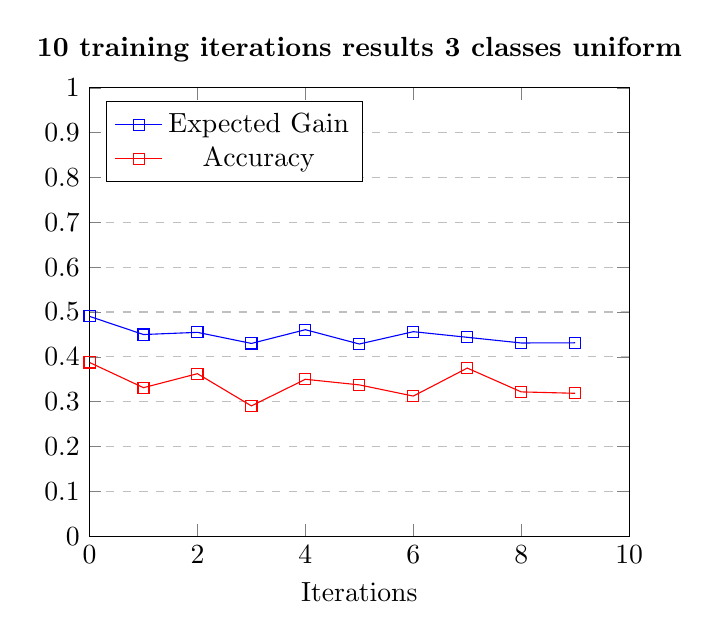
\begin{tikzpicture}
  \begin{axis}[
      title=\textbf{10 training iterations results 3 classes uniform},
      xlabel={Iterations},
      xmin=0, xmax=10,
      ymin=0.0, ymax=1,
      xtick={0,2,4,6,8,10},
      ytick={0.0,0.1,0.2,0.3,0.4,0.5,0.6,0.7,0.8,0.9,1.0},
      legend pos=north west,
      ymajorgrids=true,
      grid style=dashed,
  ]
  
  \addplot[color=blue, mark=square]
    coordinates {
      (0,0.49030720940283623)
      (1,0.44981632400021265)
      (2,0.4547041815965567)
      (3,0.42997913323401304)
      (4,0.46058465918279856)
      (5,0.4286678527092858)
      (6,0.45617940847773764)
      (7,0.44363621005504705)
      (8,0.4309883206227871)
      (9,0.43138157298087754)
    };
    \addlegendentry{Expected Gain}

  \addplot[color=red, mark=square]
    coordinates {
      (0,0.3875)
      (1,0.33125)
      (2,0.3625)
      (3,0.290625)
      (4,0.35)
      (5,0.3375)
      (6,0.3125)
      (7,0.375)
      (8,0.321875)
      (9,0.31875)
    };
    \addlegendentry{Accuracy}
      
  \end{axis}
\end{tikzpicture}